% !TeX root = ../../thesis.tex
\chapter{Fluid flow and convection}\label{ch:fluid}

\section{Introduction}


\section{Methodology}

\subsection{Navier-Stokes equations}

In its general form, the Navier-Stokes equations describing the flow of an incompressible fluid with constant density $\rho$ in the domain $\Omega \subset \mathbb{R}^{d}$ (with $d$ being the dimension so 2 or 3) can be written as \cite{Chung2014}:
\begin{equation} \label{eq:fluid_ns_general}
\left\{ {\begin{array}{*{20}{l}}
\displaystyle  {\frac{{\partial {\mathbf{u}}}}{{\partial t}} - {\nabla\cdot}[\nu(\nabla {\mathbf{u}} + \nabla {{\mathbf{u}}^T})] + ({\mathbf{u}}.\nabla ){\mathbf{u}} + \nabla {\mathbf{p}} = {\mathbf{f}},\quad x \in \Omega ,t > 0,} \\ 
\displaystyle  {\nabla\cdot{\mathbf{u}} = 0,\quad \quad \quad \quad \quad \quad \quad \quad \quad \quad \quad \quad \quad \quad x \in \Omega ,t > 0,} 
\end{array}} \right.
\end{equation}
in which $\mathbf{u}$ is the fluid velocity, $\mathbf{p}$ is the pressure (which is actually pressure divided by the density), $\nu = \frac{\mu}{\rho}$ is the kinematic viscosity (with $\mu$ being the dynamic viscosity), and 
$\mathbf{f}$ is a force term. The equations are that of conservation of linear momentum and conservation of mass (also called continuity equation), respectively. When $\nu$ is constant, the diffusion term in Eq. \ref{eq:fluid_ns_general} can be simplified as \cite{Quarteroni2014}:
\begin{equation}
\text{div} [\nu(\nabla {\bf u}+\nabla {\bf u}^{T})] =\nu (\Delta {\bf u} + \nabla \text{div} {\bf u})=\nu \Delta {\bf u},
\end{equation}
which turns Eq. \ref{eq:fluid_ns_general} into the following form:
\begin{equation}  \label{eq:fluid_ns}
\left\{ {\begin{array}{*{20}{l}}
\displaystyle  {\frac{{\partial {\mathbf{u}}}}{{\partial t}} - \nu\Delta{\mathbf{u}} + \left( {{\mathbf{u}} \cdot \nabla } \right) {\mathbf{u}} + \nabla p = {\mathbf{f}},\quad x \in \Omega ,t > 0,} \\ 
 \displaystyle {\nabla\cdot{\mathbf{u}} = 0,\quad \quad \quad \quad \quad \quad \quad \quad \quad \quad \quad \quad \quad \quad x \in \Omega ,t > 0,} 
\end{array}} \right.
\end{equation}

Eq. \ref{eq:fluid_ns} satisfies the incompressibility condition $\nabla\cdot\mathbf{u}=0$ and needs proper initial and boundary conditions to be well posed. The initial condition can be defined as:
\begin{equation}
{\bf u}({\bf x},0)={\bf u}_{0}({\bf x})\qquad \forall{\bf x}\ \epsilon\ {\bf \Omega,}
\end{equation}
where ${\bf u}_{0}$ is a divergence-free fluid field. Various types of boundary conditions can be applied, but the ones we deal with in this chapter are described here. If $\partial \Omega$ is the boundary of $\Omega$, it can be split into 3 distinct boundaries $\partial \Omega=\Gamma_{1} \cup \Gamma_{2} \cup \Gamma_{3}$ each of which with a different type. On $\Gamma_{1}$, the inlet can be defined as a Dirichlet boundary condition for the velocity for a given velocity profile ${\bf g}$:
\begin{equation}
{\bf u} = {\bf g} \quad \text{on } \Gamma_1
\end{equation}

On $\Gamma_2$, a wall boundary no-slip condition can be considered:
\begin{equation}
{\bf u} = 0 \quad \text{on } \Gamma_2
\end{equation}

On $\Gamma_3$, for the outlet condition, a homogeneous Neumann conditions on velocity and a zero pressure condition can be defined like: 
\begin{equation} \label{eq:fluid_gamma3}
\frac{\partial {\bf u}}{\partial n} = 0, \quad \mathbf{p} = 0, \quad \text{on } \Gamma_3
\end{equation}
with $n$ being the normal direction on the boundary $\partial \Omega$. Broadly speaking, these boundaries can be grouped into 2 sets: $\Gamma_{D} = \Gamma_{1} \cup \Gamma_{2}$ and $\Gamma_{N} = \Gamma_{3}$ for boundaries with Dirichlet and Neumann conditions, respectively.

The Navier-Stokes equations can be written componentwise for individual components of the flow vector field in the Cartesian coordinates. Denoting $u_i, i=1,\ldots,d$ (with $d=2$ in 2D and $d=3$ in 3D), Eq. \ref{eq:fluid_ns} can be presented as:

\begin{equation}
\left\{ {\begin{array}{*{20}{l}}
\displaystyle  {\frac{{\partial {u_i}}}{{\partial t}} - \nu \Delta {u_i} + \mathop \sum \limits_{j = 1}^d {u_j}\frac{{\partial {u_i}}}{{\partial {x_j}}} + \frac{{\partial p}}{{\partial {x_i}}} = {f_i},\qquad i = 1, \ldots ,d,} \\ 
\displaystyle  {\mathop \sum \limits_{j = 1}^d \frac{{\partial {u_j}}}{{\partial {x_j}}} = 0.} 
\end{array}} \right.
\end{equation}


\subsection{Weak formulation of the Navier-Stokes equations} \label{sec:fluid_weak}

For deriving the weak formulation, the first equation of \ref{eq:fluid_ns} is multiplied by a test function $v$ defined on a proper function space V in which the test functions vanishes on the Dirichlet boundary:
\begin{equation} \label{eq:fluid_space_v}
V = [{\bf H}^{1}_{\Gamma_{D}}(\Omega)]^{d} = \lbrace{\bf V} \in [{\bf H}^{1}(\Omega)]^{d} : {\bf v}|\Gamma_{D} = {\bf 0}\rbrace.
\end{equation}
yielding to:
\begin{equation} \label{eq:fluid_weak1}
{\mathop{\int}_{\Omega}} {\partial {\bf u} \over \partial t}.{\bf v}\ d\omega- {\mathop{\int}_{\Omega}}\nu\triangle{\bf u.v}d\omega+ {\mathop{\int}_{\Omega}}[({\bf u.\nabla){\bf u].{\bf v}}}d\omega+ {\mathop{\int}_{\Omega}}\nabla p.{\bf v}d\omega= {\mathop{\int}_{\Omega}}{\bf f. v}d\omega.
\end{equation}

\noindent Applying Green's divergence theory results in: 
\begin{equation} \label{eq:fluid_green1}
-\int_{\Omega} \nu \Delta \mathbf{u} \cdot \mathbf{v} d \omega=\int_{\Omega} \nu \nabla \mathbf{u} \cdot \nabla \mathbf{v} d \omega-\int_{\partial \Omega} \nu \frac{\partial \mathbf{u}}{\partial \mathbf{n}} \cdot \mathbf{v} d \gamma
\end{equation}
and
\begin{equation} \label{eq:fluid_green2}
\int_{\Omega} \nabla p \cdot \mathbf{v} d \omega=-\int_{\Omega} p \nabla\cdot \mathbf{v} d \omega+\int_{\partial \Omega} p \mathbf{v} \cdot \mathbf{n} d \gamma
\end{equation}

\noindent Substituting Eqs. \ref{eq:fluid_green1} and \ref{eq:fluid_green2} into Eq, \ref{eq:fluid_weak1} yields to:
\begin{equation} \label{eq:fluid_ns_weak}
\begin{array}{r}
\displaystyle\int_{\Omega} \frac{\partial \mathbf{u}}{\partial t} \cdot \mathbf{v} d \omega+\int_{\Omega} \nu \nabla \mathbf{u} \cdot \nabla \mathbf{v} d \omega+\int_{\Omega}[(\mathbf{u} \cdot \nabla) \mathbf{u}] \cdot \mathbf{v} d \omega-\int_{\Omega} p \nabla\cdot \mathbf{v} d \omega \\
\displaystyle=\int_{\Omega} \mathbf{f} \cdot \mathbf{v} d \omega+\int_{\partial \Omega}\left(\nu \frac{\partial \mathbf{u}}{\partial \mathbf{n}}-p \mathbf{n}\right) \cdot \mathbf{v} d \gamma \quad \forall \mathbf{v} \in V .
\end{array}
\end{equation}

\noindent The last term of Eq. \ref{eq:fluid_ns_weak} is expressed in accordance to the defined Neumann boundary condition, which vanishes on $\Gamma_3$ due to the defined condition in the current study (Eq. \ref{eq:fluid_gamma3}). Moreover, this term vanishes on the Dirichlet boundaries due to the properties of the function space $V$ (Eq. \ref{eq:fluid_space_v}).

Similarly, the second equation of \ref{eq:fluid_ns} is multiplied by a test function $q$ belonging to the function space Q, called the pressure space: 
\begin{equation}
Q = {\bf L}^2_0(\Omega) = \lbrace p \in L^2(\Omega) : {\mathop{\int}_{\Omega}} p \ d\omega = 0\rbrace,
\end{equation}
resulting in:
\begin{equation} \label{eq:fluid_ns_weak_pressure}
{\mathop{\int}_{\Omega}} q \nabla\cdot{\bf u}\ d\omega = 0 \qquad \forall q \in Q.
\end{equation}

Eqs. \ref{eq:fluid_ns_weak} and \ref{eq:fluid_ns_weak_pressure} are so called weak forms of the Navier-Stokes equations. 

\subsection{Stokes equations}

For viscous flow, where the Reynolds number is less than 1 ($Re = {|{\bf U}|L \over \nu}$, with $L$ and $\bf U$ being the representative length and velocity of the domain), the convection term of the Navier-Stokes equations can be neglected, simplifying Eq. \ref{eq:fluid_ns} to \cite{Quarteroni2014}:
\begin{equation} \label{eq:fluid_stokes}
\left\{ {\begin{array}{*{20}{l}}
\displaystyle  {\alpha \mathbf{u} - \nu\Delta \mathbf{u} + \nabla p = f\quad \text{in}\;\Omega ,} \\ 
\displaystyle  {\nabla\cdot\mathbf{u} = 0\quad \quad \quad \quad \;\;\;\text{in}\;\Omega ,}
\end{array}} \right.
\end{equation}
with $\alpha$ being a positive coefficient. Eq. \ref{eq:fluid_stokes} can be used to model laminar flow in low Reynolds regimes and is simpler to handle than Eq. \ref{eq:fluid_ns} from the numerical computing perspective. The weak formulation of the Stokes equation can be derived by following the approach taken for the Navier-Stokes equations in Section \ref{sec:fluid_weak}. The final form of the weak formulation is:
\begin{equation} \label{eq:fluid_stokes_weak}
\left\{ {\begin{array}{*{20}{l}}
\displaystyle  {\int\limits_\Omega  {(\alpha {\mathbf{u}}.{\mathbf{v}} + \nu\nabla {\mathbf{u}}.\nabla {\mathbf{v}})\,} d\omega  - \int\limits_\Omega  {p\nabla\cdot{\mathbf{v}}\;d\omega  = } \int\limits_\Omega  {{\mathbf{f}}.{\mathbf{v}}\;d\omega \qquad {\forall {\mathbf{v}}} \in V,} } \\ 
\displaystyle  {\int\limits_\Omega  {q\nabla\cdot{\mathbf{u}}\;d\omega  = 0} \qquad \qquad \qquad \qquad \qquad \qquad \qquad \;\;\;{\forall {{q}}} \in Q,} 
\end{array}} \right.
\end{equation}

Eq. \ref{eq:fluid_stokes_weak} can be written in the standard finite element variational form by defining 2 bilinear terms $a: V \times V \mapsto \mathbb{R}$ and $b: V \times Q \mapsto \mathbb{R}$:
\begin{equation}
\begin{array}{*{20}{l}}
\displaystyle  {a({\mathbf{u}},{\mathbf{v}}) = \int\limits_\Omega  {(\alpha {\mathbf{u}}.{\mathbf{v}} + \nu\nabla {\mathbf{u}}.\nabla {\mathbf{v}})\;d\omega ,} } \\ 
\displaystyle  {b({\mathbf{u}},{\mathbf{q}}) =  - \int\limits_\Omega  {q\nabla\cdot{\mathbf{u}}\;d\omega ,} } 
\end{array}
\end{equation}
which causes the variational problem of the the Stokes equation becomes to find $(\mathbf{u}, p) \in V \times Q$ such that
\begin{equation}
\left\{ {\begin{array}{*{20}{l}}
\displaystyle  {a({\mathbf{u}},{\mathbf{v}}) + {\mathbf{b}}({\mathbf{v}},{\mathbf{p}}) = ({\mathbf{f}},{\mathbf{v}})\qquad {\forall {\mathbf{v}}} \in V,} \\ 
\displaystyle  {b({\mathbf{u}},{\mathbf{q}}) = 0\qquad \qquad \qquad \quad \;{\forall {\mathbf{q}}} \in Q,} 
\end{array}} \right.
\end{equation}
in which
\begin{equation}
(\mathbf{f}, \mathbf{v})=\sum_{i=1}^{d} \int_{\Omega} f_{i} v_{i} d \omega.
\end{equation}


\subsection{Implementation}

Numerical implementation of the Stokes (Eq. \ref{eq:fluid_stokes}) and Navier-Stokes (Eq. \ref{eq:fluid_stokes}) equations can be tricky due to presence of certain sources of instability, which highly depends on the type of studied fluid regime \cite{Girault1979, Elman2014}. Various numerical models have presented for dealing with these equations, some of which are commonly used in CFD applications, such as the Newton-Raphson approximation of Navier-Stokes equtaions and the Chorin's projection method. 

In order to increase the stability and avoid some problems on the mathematical analysis of the numerical models (V-ellipticity
property), a pseudo-compressibility assumption can be added to the continuity equation. The pseudo-compressible approximation appears as a pressure term $\varepsilon p$ with $\varepsilon$ being a very small coefficient, resulting to the following equation as the final form of the Navier-Stokes equations we consider in this study \cite{devuyst2013}:
\begin{equation}  \label{eq:fluid_ns_pseudo}
\left\{ {\begin{array}{*{20}{l}}
\displaystyle  {\frac{{\partial {\mathbf{u}}}}{{\partial t}} - \nu\Delta{\mathbf{u}} + \left( {{\mathbf{u}} \cdot \nabla } \right) {\mathbf{u}} + \nabla p = {\mathbf{f}},} \\ 
 \displaystyle {\nabla\cdot{\mathbf{u}} + \varepsilon p = 0.} 
\end{array}} \right.
\end{equation}

Similarly, the Stokes equation can be written as:
\begin{equation} \label{eq:fluid_stokes_pseudo}
\left\{ {\begin{array}{*{20}{l}}
\displaystyle  {\alpha \mathbf{u} - \nu\Delta \mathbf{u} + \nabla p = f,} \\ 
\displaystyle  {\nabla\cdot\mathbf{u} + \varepsilon p = 0.}
\end{array}} \right.
\end{equation}

Another challenging part is to approximate the convection terms in the equations. One of the best approaches to do so is to take advantage of the method of characteristics, in which the characteristics curves of a PDE are used to convert it to an ODE, resulting to a simpler solution. By using the method of characteristics for the convection term and a backward Euler discretization for the temporal term, the weak form of the Navier-Stokes and continuity equations (Eq. \ref{eq:fluid_ns_weak} and \ref{eq:fluid_ns_weak_pressure}) can be rewritten as:
\begin{equation} \label{eq:fluid_ns_weak_implement}
\begin{aligned}
&\int_{\Omega} \frac{\mathbf{u}^{n+1}-\mathbf{u}^{n} \circ X^{n}}{\Delta t} \cdot \mathbf{v} d \omega+\nu \int_{\Omega} \nabla \mathbf{u}^{n+1} \cdot \nabla \mathbf{v} d \omega-\int_{\Omega} p^{n+1} \nabla \cdot \mathbf{v} d \omega=\int_{\Omega} \boldsymbol{f} \cdot \mathbf{v} d\omega \\
&\int_{\Omega} \nabla \cdot \mathbf{u}^{n+1} q d \omega+\varepsilon \int_{\Omega} p^{n+1} q d \omega=0
\end{aligned}
\end{equation}
in which $(\mathbf{u}^{n+1},p^{n+1})$ are unknowns to be computed from the known state $\mathbf{u}^{n}$ coming from the previous time step or the initial condition. In Eq. \ref{eq:fluid_ns_weak_implement}, the term $\mathbf{u}^{n+1}-\mathbf{u}^{n} \circ X^{n}$ is corresponding to the convection term being approximated using the method of characteristics.

The weak form of the Stokes equations stays almost the same as Eq. \ref{eq:fluid_stokes_weak} (because it doesn't contain transient and convection terms) but needs a slight modification to add the pseudo-compressible terms from Eq. \ref{eq:fluid_stokes_pseudo}:
\begin{equation} \label{eq:fluid_stokes_weak_implement}
\begin{array}{*{20}{l}}
\displaystyle  {\int\limits_\Omega  {(\alpha {\mathbf{u}}.{\mathbf{v}} + \nu\nabla {\mathbf{u}}.\nabla {\mathbf{v}})\,} d\omega  - \int\limits_\Omega  {p\nabla\cdot{\mathbf{v}}\;d\omega  = } \int\limits_\Omega  {{\mathbf{f}}.{\mathbf{v}}\;d\omega,} } \\ 
\displaystyle  {\int\limits_\Omega  {q\nabla\cdot{\mathbf{u}}\;d\omega +\varepsilon \int_{\Omega} p q d \omega  = 0}.} 
\end{array}
\end{equation}

\subsection{Considering the degrading object}

In biodegradation simulations, a degrading object exists in the fluid domain, through which the flow should not pass because it is a solid part. One common approach to handle this situation is to remove the solid part from the fluid flow mesh, but since the part shrinks over time, this is not a feasible and efficient approach, needing tremendous mesh recreation and removal during simulation. As a result, in the current study, presence of the solid body as a barrier is taken into account by adding a Darcy term for the permeability to the Navier-Stokes and Stokes and equations. A penalization technique is then employed to implement it in the weak formulation. To couple the fluid flow model with the biodegradation model, a convection term is added to the ions transport equations, causing the ions be advected by the fluid velocity field.

Adding the Darcy  term to Eq. \ref{eq:fluid_stokes} and considering no other acting force yields to:
\begin{equation} \label{eq:fluid_stokes_permeab}
- \nu\Delta \mathbf{u} + \nabla p + \frac{\nu}{K} \mathbf{u} = 0,
\end{equation}
where $K$ is the permeability function. The Darcy term vanishes in regions with high permeability, i.e. inside the fluid domain, resembling the Stokes equation, but when $K$ is very small, i.e. inside the solid part, it dominates the flow and acts like a barrier. To avoid numerical perturbation for switching between these 2 regions, a heaviside function is defined to update $K$ \cite{Guyot2016}:
\begin{equation}
H(\phi)=\left\{\begin{array}{l}
0, \quad \phi<-\varepsilon \\
\frac{1}{2}+\frac{\phi}{2 \varepsilon}+\frac{1}{2 \pi} \sin \left(\frac{\pi \phi}{\varepsilon}\right), \quad-\varepsilon<\phi<\varepsilon \\
1, \quad \phi>-\varepsilon
\end{array}\right.
\end{equation}
in which $\phi$ is the level-set signed distance function used to separate the solid and solution parts (Eqs. \ref{eq:lsm_full} and \ref{eq:lsm_simplified}), and $\varepsilon$ is set to 1.5h, with h being the minimum mesh element size. Then, $K$ can be accordingly updated to have smooth transition between regions with big difference in permeability:
\begin{equation}
K(\boldsymbol{x})=10^{30}(1-H)+K_{0} H
\end{equation}
where $K_{0}$ is the permeability of metals in fluid regions ($\sim10^{-6}$ H/m).



Eqs. \ref{eq:fluid_ns_weak_implement} and \ref{eq:fluid_stokes_weak_implement} can be easily implemented in FreeFEM thanks to the built-in support of the method of characteristics via the \verb|convect| function. The model is implemented using P1 elements for the pressure and P2 elements for the velocity state variables.



\begin{figure}[h]
\centering
\medskip
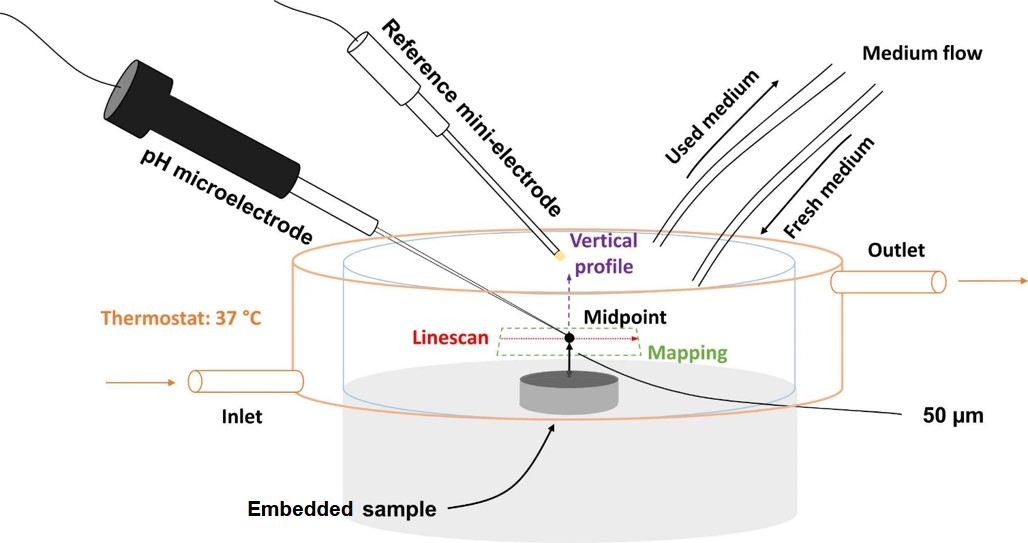
\includegraphics[width=\textwidth]{setup.jpg}
\caption[Fluid flow model construction for comparison with experimental setup]{Fluid flow model construction for comparison with experimental setup} \label{fig:fluid_setup}
\end{figure}

\begin{figure}[h]
\centering
\medskip
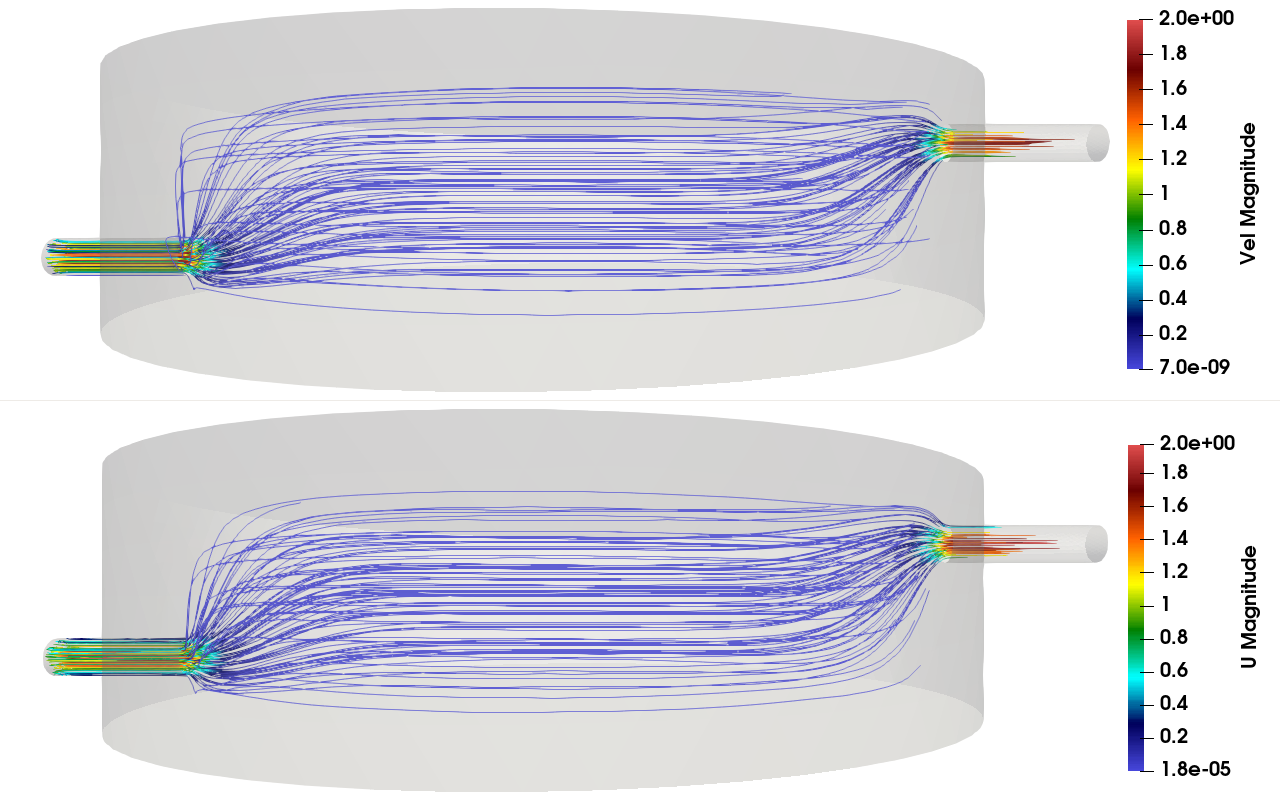
\includegraphics[width=\textwidth]{streamlines_side.png}
\caption[Comparing streamline results of developed CFD code and OpenFOAM - side view]{Comparing streamline results of developed CFD code and OpenFOAM - side view} \label{fig:fluid_streamlines_side}
\end{figure}


\begin{figure}[h]
\centering
\medskip
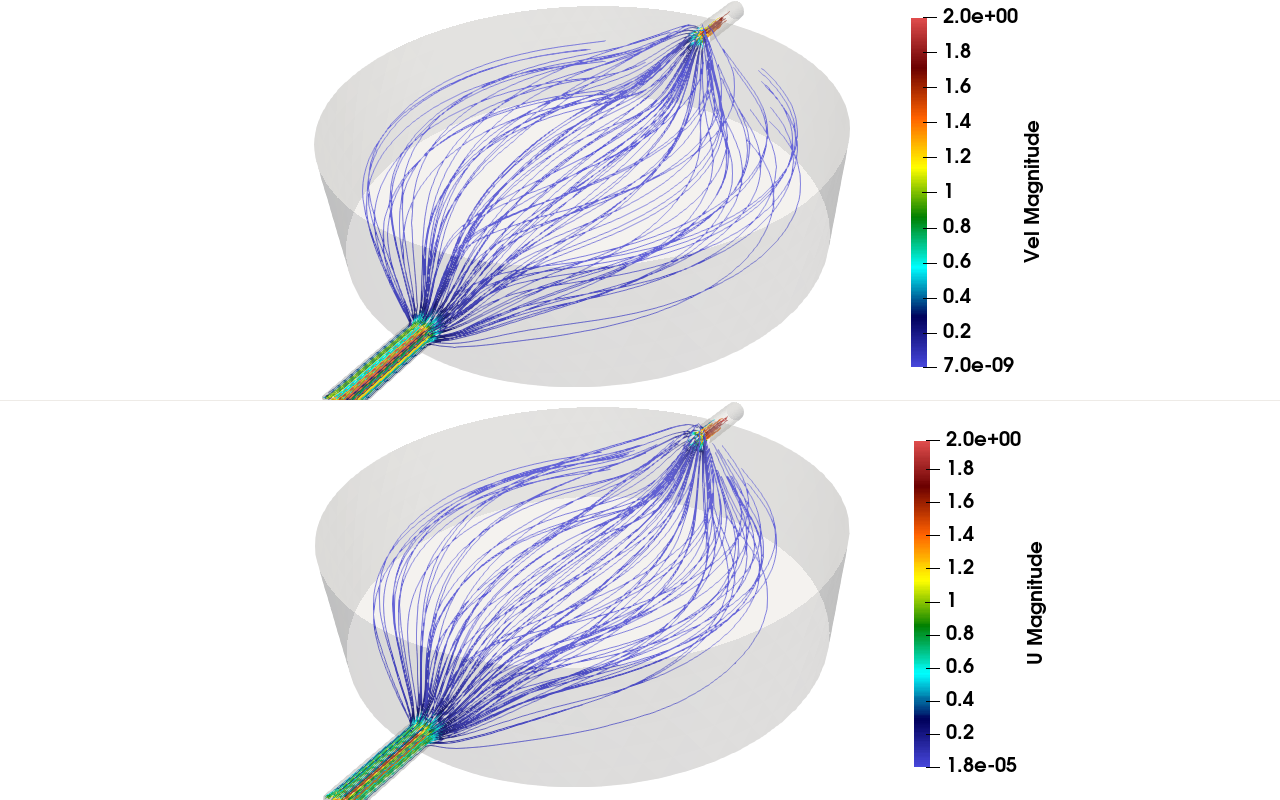
\includegraphics[width=\textwidth]{streamlines_top.png}
\caption[Comparing streamline results of developed CFD code and OpenFOAM - top view]{Comparing streamline results of developed CFD code and OpenFOAM - top view} \label{fig:fluid_streamlines_top}
\end{figure}


\begin{figure}[h]
\centering
\medskip
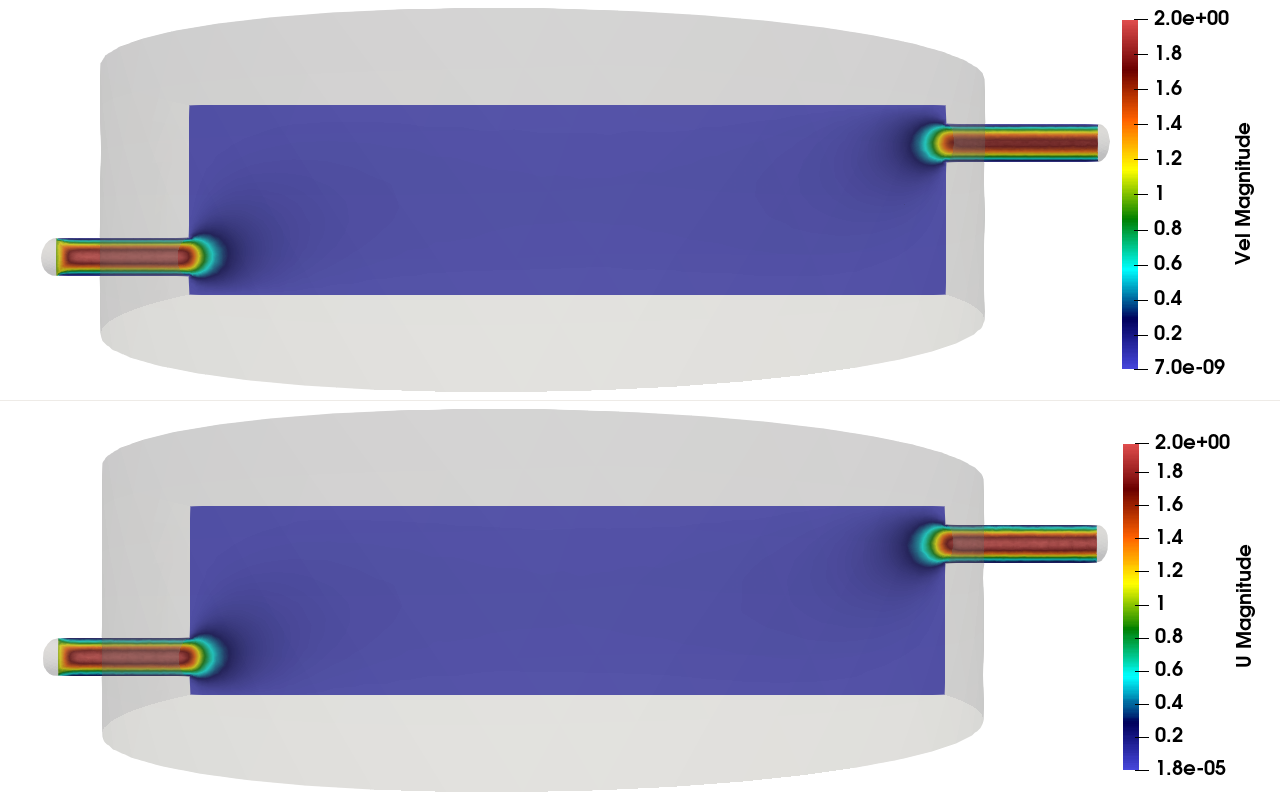
\includegraphics[width=\textwidth]{flow_chamber.png}
\caption[Comparing flow field results of developed CFD code and OpenFOAM]{Comparing streamline results of developed CFD code and OpenFOAM} \label{fig:fluid_flow_chamber}
\end{figure}


\begin{figure}[h]
\centering
\medskip
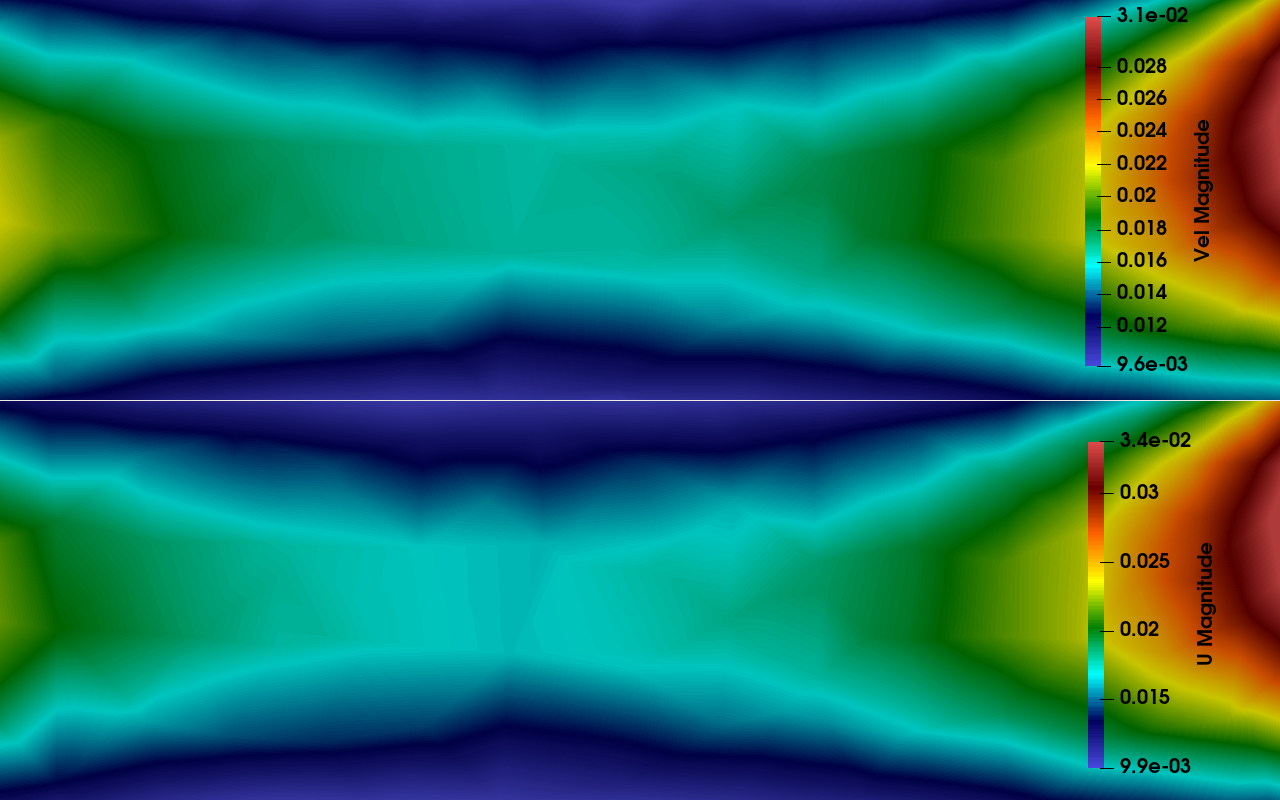
\includegraphics[width=\textwidth]{flow_chamber_zoom.png}
\caption[Comparing flow field results of developed CFD code and OpenFOAM - zoomed view]{Comparing streamline results of developed CFD code and OpenFOAM - zoomed view} \label{fig:fluid_flow_chamber_zoom}
\end{figure}

\begin{figure}[h]
\centering
\medskip
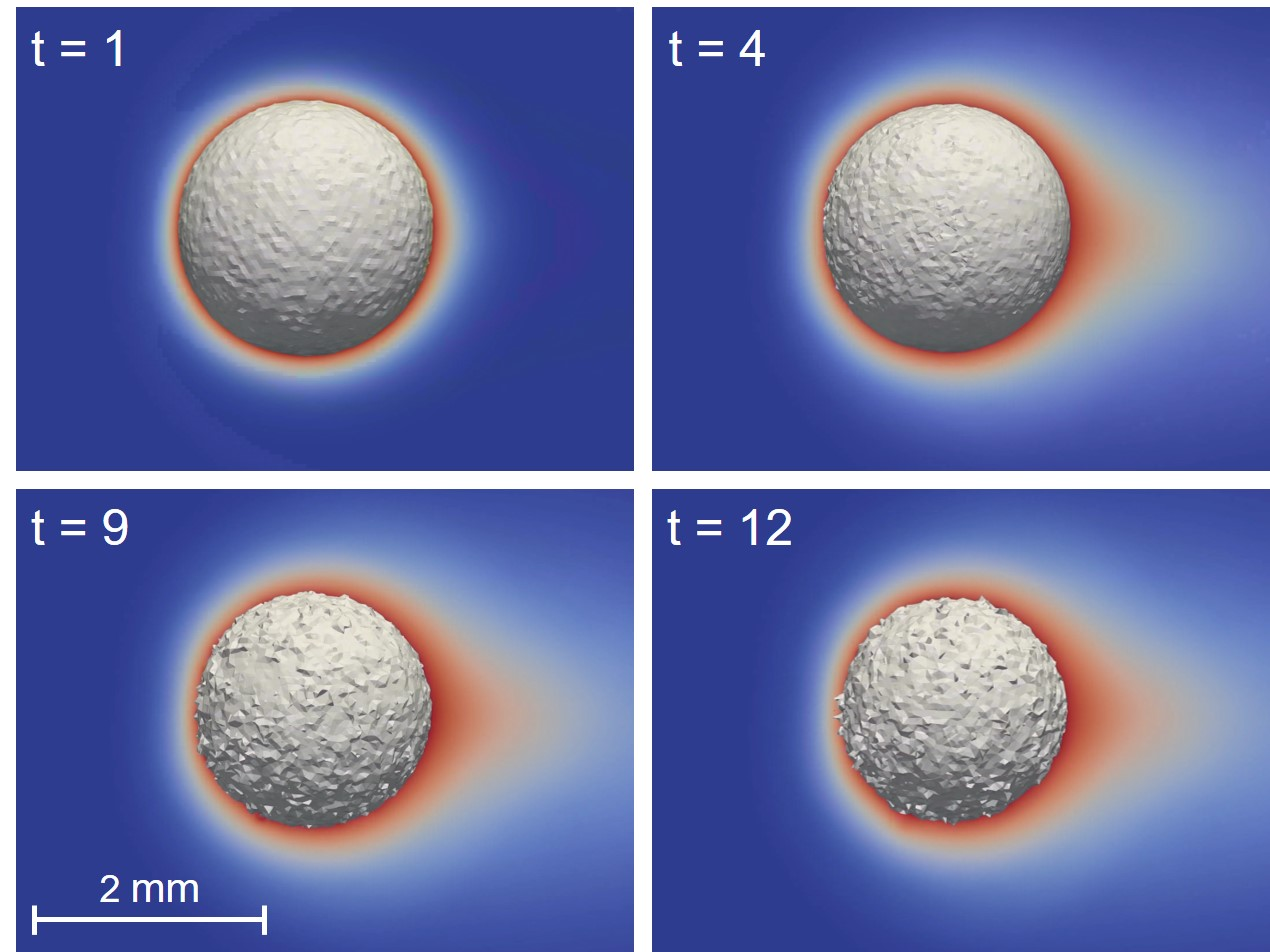
\includegraphics[width=\textwidth]{flow_degrading.jpg}
\caption[Biodegradation simulation results in the presence of fluid flow]{Biodegradation simulation results in the presence of fluid flow} \label{fig:fluid_flow_degrading}
\end{figure}


\begin{figure}[h]
\centering
\medskip
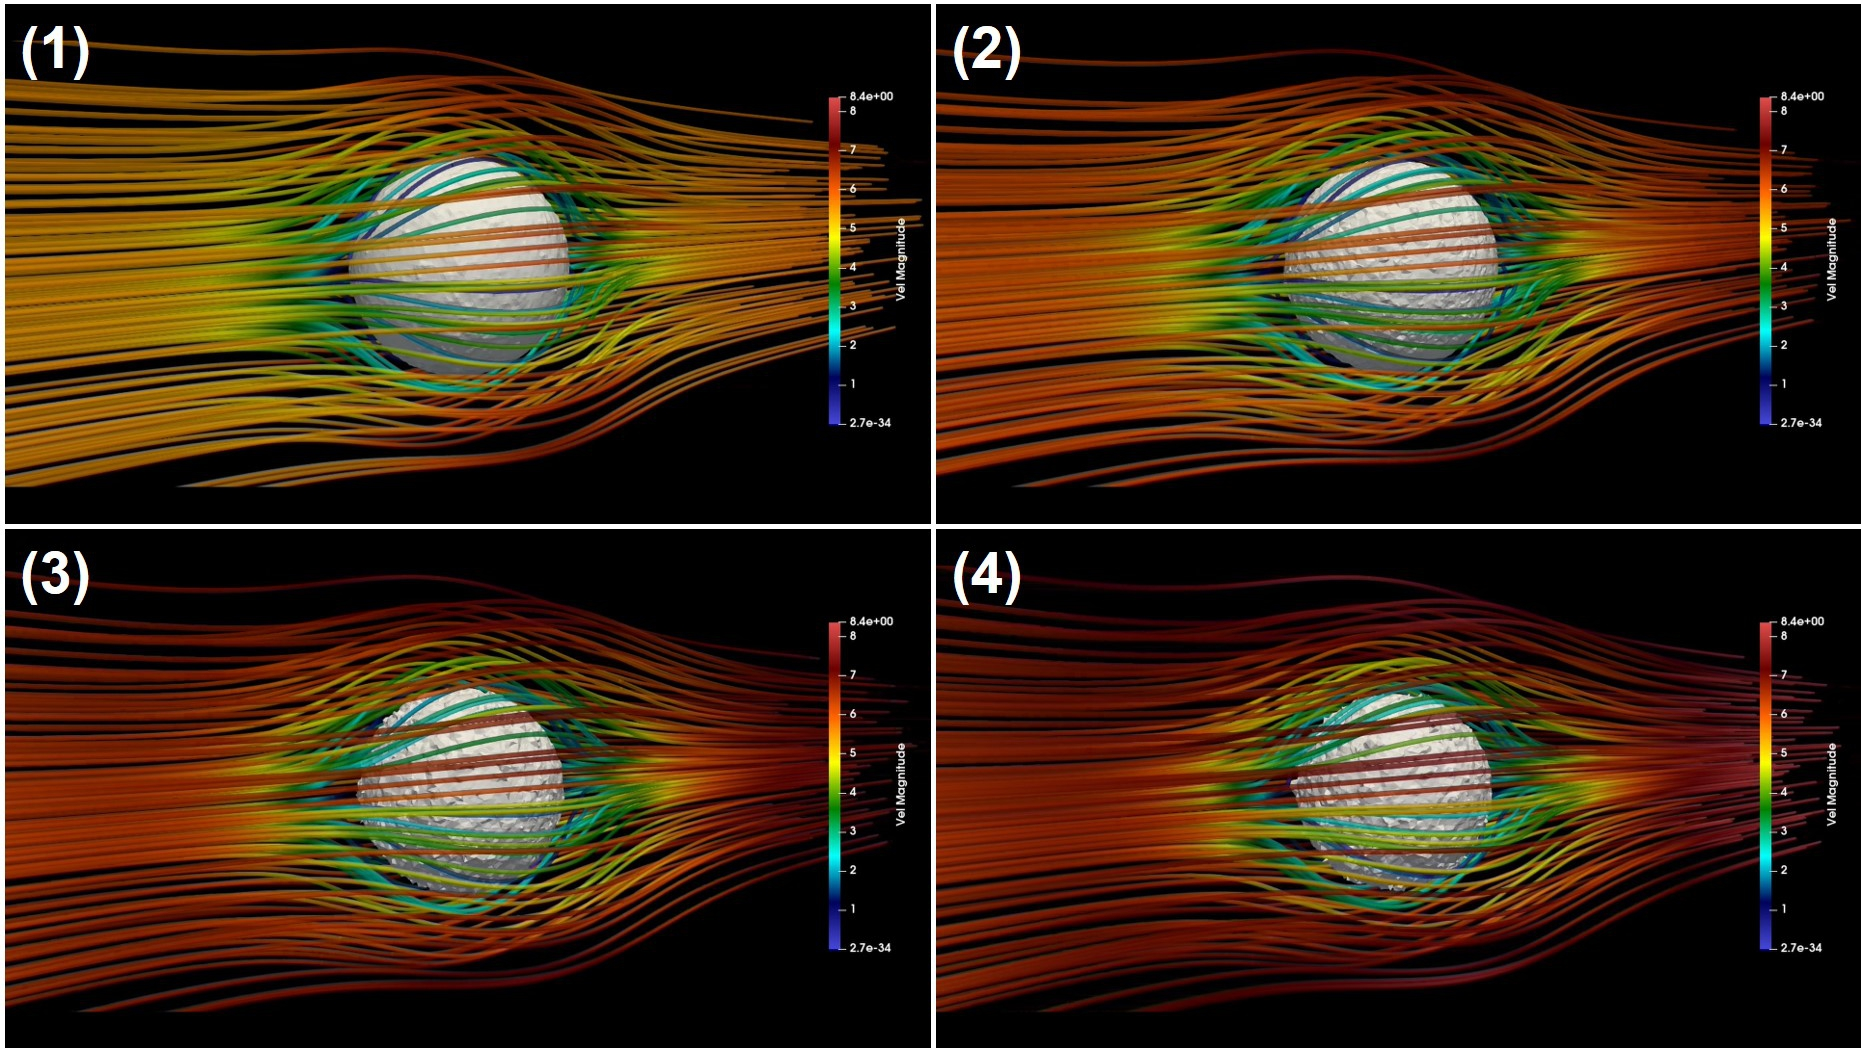
\includegraphics[width=\textwidth]{flow_degrading_streamline.jpg}
\caption[Fluid flow streamlines in the presence of a degrading object]{Fluid flow streamlines in the presence of a degrading object} \label{fig:fluid_flow_degrading_streamline}
\end{figure}
















%%%%%%%%%%%%%%%%%%%%%%%%%%%%%%%%%%%%%%%%%%%%%%%%%%
% Keep the following \cleardoublepage at the end of this file, 
% otherwise \includeonly includes empty pages.
\cleardoublepage

